\documentclass[../norme-di-progetto.tex]{subfiles}
\begin{document}

%%%%%%%%%%%%%%%%%%%%%%%%%%%%
%%% 3.1 - DOCUMENTAZIONE %%%
%%%%%%%%%%%%%%%%%%%%%%%%%%%%
\subsection{Documentazione}
\subsubsection{Scopo}
Lo scopo del processo di documentazione è quello di fornire i dettagli e le regole su cui deve essere basata la redazione e la manutenzione di tutta la documentazione durante l'intero \glossario{ciclo di vita} del software.

\subsubsection{Aspettative}
Le aspettative della corretta implementazione di questo processo sono:
\begin{itemize}
  \item L'identificazione di regole su cui deve essere basata la corretta stesura dei documenti;
  \item L'individuazione di una struttura rigorosa sulla quale basare la redazione dei documenti durante tutti i processi di sviluppo.
\end{itemize}

\subsubsection{Descrizione}
Questa sezione descrive i dettagli su come deve essere redatta e verificata la documentazione. Al fine di ottenere l'uniformità e il rigore espositivo di tutti i documenti prodotti durante il ciclo di vita del software, ogni documento deve basarsi sulle regole descritte in questa sede.

\subsubsection{Attività}
\paragraph{Implementazione del processo}
\subparagraph{Ciclo di vita dei documenti}
Il documento viene innanzitutto creato; a tale scopo, il gruppo ha deciso di creare un template \LaTeX\ sul quale basare la stesura di ogni documento. Questo assicura l'uniformità della struttura dei documenti, facilitando inoltre il \glossario{versionamento}. \\
Dopo la creazione, il ciclo di vita dei documenti è suddiviso in tre differenti attività:
\begin{itemize}
  \item \textbf{Stesura del documento}: la stesura del documento consiste nella scrittura del documento stesso. Questa attività viene svolta da un redattore, assegnato dal Responsabile di progetto; dopo la stesura, il Responsabile autorizzerà all'avanzamento della stesura, rimanendo in attesa dell'esito della revisione;
  \item \textbf{Revisione}: dopo la stesura, il documento verrà revisionato dai Verificatori, che ne controlleranno l'aderenza alle norme di progetto e la correttezza sintattica e semantica. Dopo questo controllo, a seconda che l'esito sia positivo o negativo, lo comunicheranno al Responsabile, che farà avanzare il documento all'approvazione finale, o ai Redattori, che correggeranno eventuali segnalazioni e lo riproporranno ai Verificatori;
  \item \textbf{Approvazione finale}: con l'approvazione ricevuta da parte dei Verificatori, il Responsabile di progetto confermerà quindi il documento, eseguendone il rilascio.
\end{itemize}

\subparagraph{Struttura dei documenti}
Al fine di organizzare coerentemente e uniformemente la struttura dei documenti, si è deciso di utilizzare il \textit{package} \textbf{subfiles} di \LaTeX. La \glossario{repository} contiene una \textit{directory} denominata \texttt{commons/} con al suo interno:
\begin{itemize}
  \item Il file \texttt{config.tex}, contenente le definizioni dei comandi \LaTeX;
  \item Il file \texttt{template.tex}, contenente il \textit{template} su cui si basano tutti i documenti;
  \item La cartella \texttt{img/}, contenente le immagini comuni a tutti i documenti.
\end{itemize}
Per ogni documento è quindi presente una \textit{directory} contenente:
\begin{itemize}
  \item  Il file principale, chiamato con il nome del documento, in formato \texttt{.tex};
  \item La cartella \texttt{components/}, contenente gli altri file in formato \texttt{.tex} che vengono inclusi nel file principale ed eventuali allegati interni al documento.
\end{itemize}
Basandosi su un \textit{template}, ogni documento ha quindi una struttura fissa e predeterminata.

\subparagraph*{Frontespizio}
Il frontespizio fornisce tutti i dati principali del documento. Esso presenta il logo del gruppo, centrato, seguito dal nome del gruppo e dal titolo del progetto; sotto di questo è presente il titolo del documento. \\
Sono fornite anche altre informazioni essenziali, le quali sono:
\begin{itemize}
  \item \textbf{Versione}: versione attuale del documento;
  \item \textbf{Approvazione}: stato di approvazione del documento, che può essere "In redazione" o indicare il nome del responsabile che ha approvato il documento;
  \item \textbf{Redazione}: redattori del documento;
  \item \textbf{Verifica}: verificatori del documento;
  \item \textbf{Uso}: destinazione del documento, che può essere "Interno" o "Esterno";
  \item \textbf{Destinato a}: destinazione specifica del documento.
\end{itemize}
\subparagraph*{Registro delle modifiche}
Nella seconda pagina di ogni documento è presente il registro delle modifiche del documento, consistente in una tabella contentente, per ogni modifica:
\begin{itemize}
  \item \textbf{Versione}: la versione del documento aggiornata alla modifica effettuata;
  \item \textbf{Nominativo}: il nome dell'autore della modifica;
  \item \textbf{Ruolo}: il ruolo dell'autore della modifica;
  \item \textbf{Data}: la data in cui è stata effettuata la modifica;
  \item \textbf{Descrizione}: la descrizione della modifica effettuata.
\end{itemize}
\subparagraph*{Indice}
L'indice riepiloga la struttura del documento. Ha una struttura standard: la numerazione ha struttura \begin{center}
  \centering
  \textbf{a.b.c.d.e}
\end{center} dove:
\begin{itemize}
  \item \textbf{a} è il capitolo principale;
  \item \textbf{b} è la sezione del capitolo;
  \item \textbf{c} è la sottosezione della sezione;
  \item \textbf{d} è il paragrafo della sezione;
  \item \textbf{e} è il sottoparagrafo del paragrafo.
\end{itemize}
La massima profondità della numerazione è quindi 5; nel caso in cui si rendesse necessario aggiungere un livello, questo verrà indicato come sottoparagrafo del sottoparagrafo senza ulteriore numerazione.

\subparagraph*{Elenco delle figure}
L'elenco delle figure consiste nell'indice di tutte le figure presenti nel documento, eccezion fatta per il logo del gruppo che non viene riportato. L'elenco riporta il numero della figura, il nome descrittivo e la pagina in cui si trova.

\subparagraph*{Elenco delle tabelle}
L'elenco delle tabelle indicizza tutte le tabelle presenti nel documento, esclusa quella del Registro delle modifiche. L'elenco riporta il numero della tabella, il nome  descrittivo e la pagina in cui si trova.

\subparagraph*{Contenuto principale}
Ogni pagina del contenuto principale del documento è composta da:
\begin{itemize}
  \item Il logo del gruppo, posizionato in alto a sinistra;
  \item Il nome del gruppo, posizionato in alto a destra;
  \item Il nome del documento, posizionato in alto a destra sotto al nome del gruppo;
  \item Una riga orizzontale, posizionata in alto e che attraversa tutta la pagina, che divide logo, nome del gruppo e nome del documento dal contenuto della pagina;
  \item Il numero di pagina, posizionato in basso a destra e nel formato \\ \begin{center}
    \centering
    \textbf{N di T}
  \end{center} dove
\begin{itemize}
  \item \textbf{N} è il numero della pagina corrente;
  \item \textbf{T} è il numero di pagine totali.
\end{itemize}
Il conteggio delle pagine inizia dalla prima pagina dopo l'Elenco delle tabelle.
\end{itemize}
Nello spazio compreso tra la riga orizzontale e il numero di pagina si articola il contenuto proprio della pagina.

\subparagraph{Classi di documenti}
I documenti prodotti appartengono a diverse categorie, secondo le quali sono classificati.

\subparagraph*{Documenti ufficiali}
I documenti ufficiali sono quelli che seguono la struttura elencata in questo documento, e che sono stati verificati e approvati dal responsabile di progetto. Essi possono essere Interni o Esterni, a seconda della destinazione che hanno. I documenti ufficiali sono i seguenti:

\subparagraph*{Glossario}
In accompagnamento ai documenti ufficiali viene fornito un \textsc{Glossario v2.0.0}, contenente tutti i termini caratterizzati da sottolineatura e una G maiuscola come pedice. Il glossario ha la funzione di chiarire possibili fraintendimenti provenienti dall'utilizzo di determinati termini. \\
Perché un termine venga incluso nel glossario deve soddisfare almeno uno tra i seguenti requisiti:
\begin{itemize}
  \item Essere un termine tecnico. Rientrano in questo criterio i nomi propri delle tecnologie utilizzate, i termini tecnici propri di queste e i termini frequentemente utilizzati nell'Ingegneria del Software;
  \item Essere presente in tutti i documenti;
  \item Avere più di un significato plausibile nel contesto in cui viene utilizzato;
  \item Essere un acronimo specifico e raramente usato.
\end{itemize}
Il \textsc{Glossario v1.0.0} possiede un'impostazione grafica identica agli altri documenti, con l'eccezione di non possedere numerazione nell'indice. I termini sono ordinati in ordine alfabetico, e divisi in base alla prima lettera; ogni lettera deve avere la sua sezione, anche nel caso in cui nessun termine vi appartenga. \\
I termini appartenenti al glossario sono contrassegnati come tali solo una volta per ogni documento, nello specifico la prima volta che il termine compare in esso, al fine di evitare l'appesantimento visivo.

\subparagraph*{Verbali}
I verbali documentano gli argomenti discussi in una riunione; essi possono essere interni, e quindi riferirsi a una riunione tra soli membri del gruppo, o esterni, e quindi riferirsi a una riunione a cui partecipa anche il proponente e/o il committente. La struttura del documento è identica a quella dei documenti ufficiali. \\
Ogni verbale è composto dai seguenti componenti:
\begin{itemize}
  \item \textbf{Informazioni generali}: informazioni dell'incontro, consistenti nella modalità, nella data e negli orari di inizio e fine, e i partecipanti all'incontro;
  \item \textbf{Ordine del giorno}: lista degli argomenti e dei temi di cui il gruppo ha deciso di discutere durante l'incontro;
  \item \textbf{Resoconto}: riassunto di quanto detto durante l'incontro punto per punto;
  \item \textbf{Tracciamento delle decisioni}: tabella contenente il riassunto delle decisioni prese dal gruppo durante l'incontro.
\end{itemize}

\subparagraph*{Lettere}
Le lettere, tra cui quella di presentazione, seguono il formato classico di una lettera: esse includono quindi uno o più mittenti e uno o più destinatari, il logo e il nome del gruppo. \\
La lettera di presentazione contiene anche l'elenco dei documenti rilasciati e il preventivo per lo svolgimento del progetto.

\subparagraph*{Documenti ufficiosi}
Il gruppo si avvale anche dello strumento Google Docs per la condivisione immediata di idee e proposte da parte dei componenti del gruppo. Questo meccanismo funge solo da supporto all'organizzazione delle idee del gruppo; nessun documento ufficioso deve essere utilizzato come documento ufficiale o come parte di esso.

\subparagraph{Norme tipografiche}
\subparagraph*{Nomi dei file}
La nomenclatura di tutti i file segue la convenzione \glossario{kebab case}, nota anche come \textit{lisp-case}. Le regole di questa convenzione sono le seguenti:
\begin{itemize}
  \item Ogni file inizia con una lettera minuscola;
  \item Tra ogni parola viene inserito come separatore il tratto d'unione \textbf{-};
  \item In caso di presenza di apostrofo, esso verrà sostituito dal tratto d'unione;
  \item Le lettere accentate sono abolite, sostituite dalla semplice lettera senza accento.
\end{itemize}
L'unica eccezione che è stata adottata è l'utilizzo del segno di interpunzione "trattino basso" \textbf{\_} tra il nome del documento e la data di redazione nei nomi dei verbali e tra la data e la versione del documento. \\
Tutti i nomi di file avranno quindi il seguente formato: \\ \begin{center}
  \centering
  \textbf{N-a-b-c[\_YYYY-MM-DD]\_vX.Y.Z.ext}
\end{center} dove:
\begin{itemize}
  \item \textbf{N} è il numero di verbale nel caso in cui il documento sia un verbale; opzionalmente, può essere utilizzato per numerare ordinatamente i \textit{subfiles} di un determinato documento;
  \item Le parentesi quadre \textbf{[ ]} si applicano solo al caso dei verbali;
  \item \textbf{a}, \textbf{b} e \textbf{c} sono parole singole. Il numero di parole singole non è limitato a tre ma si può aumentare o diminuire. Nel caso specifico dei verbali, la forma di questa porzione di nome è \\ \begin{center}
    \centering
    \textbf{verbale-[interno/esterno]}
  \end{center};
  \item \textbf{vX.Y.Z} indicano la versione attuale del documento;
  \item \textbf{ext} è l'estensione del file.
\end{itemize}
Alcuni esempi di nomi di files legittimi sono quindi:
\begin{itemize}
  \item \texttt{1-verbale-interno\_2020\_01\_13\_v1.0.0.tex};
  \item \texttt{norme-di-progetto.tex}, con annessi \textit{subfiles}:
    \begin{itemize}
      \item \texttt{1-introduzione.tex};
      \item \texttt{2-processi-primari.tex};
      \item \texttt{3-processi-supporto.tex};
      \item \texttt{4-processi-organizzativi.tex}.
    \end{itemize}
\end{itemize}

\subparagraph*{Stile del testo}
Ogni diversa formattazione usata all'interno dei documenti ha un significato preciso, e ogni documento deve obbligatoriamente seguire questo stile. Gli stili sono:
\begin{itemize}
  \item Utilizzo di testo in corsivo per i termini in lingua diversa da quella italiana non inclusi nel glossario;
  \item Utilizzo di testo in caratteri dattilografici per i nomi di file e delle \textit{directories}; queste ultime devono finire con il carattere barra \textbf{/};
  \item Utilizzo di testo in grassetto per i termini conseguentemente definiti e per i titoli dei sottoparagrafi di sottoparagrafi. Viene inoltre utilizzato per rimarcare concetti considerati importanti;
  \item Utilizzo di testo sottolineato, in aggiunta al pedice G maiuscola, per i termini appartenenti al \textsc{Glossario};
  \item Utilizzo di testo maiuscoletto per i nomi dei documenti all'interno dei documenti stessi.
\end{itemize}

\subparagraph*{Figure}
L'utilizzo di figure all'interno dei documenti è permesso; le immagini devono essere centrate nella pagina, avere larghezza o lunghezza massima di 15cm ed essere seguite dalla seguente dicitura: \\ \begin{center}
  \centering
  \textbf{Figura N: D}
\end{center} dove:
\begin{itemize}
  \item \textbf{N} è il numero progressivo della figura all'interno del documento in cui è inserita;
  \item \textbf{D} è una breve descrizione dell'immagine.
\end{itemize}
Il logo del gruppo non segue queste regole, poiché non possiede né numero progressivo né descrizione.

\subparagraph*{Diagrammi UML}
Tutti i diagrammi UML sono inseriti nei documenti come figure, e come tali figurano nell'Elenco delle Figure.

\subparagraph*{Tabelle}
L'utilizzo delle tabelle è permesso e incoraggiato nel caso in cui permettano una più facile visualizzazione di un insieme di dati. \\
Le tabelle devono essere centrate nella pagina, ed essere seguite dalla seguente dicitura: \\ \begin{center}
  \centering
  \textbf{Tabella N: D}
\end{center} dove:
\begin{itemize}
  \item \textbf{N} è il numero progressivo della tabella all'interno del documento in cui è inserita;
  \item \textbf{T} è il titolo della tabella.
\end{itemize}
La tabella del Registro delle modifiche non segue queste regole, poiché non possiede né numero progressivo né titolo.

\subparagraph*{Formati comuni}
I formati di data, ora e versione sono determinati e univoci per ogni documento. Nello specifico:
\begin{itemize}
  \item La data segue lo standard \textbf{ISO 8601}, e quindi è nel formato \\ \begin{center}
    \centering
    \textbf{YYYY-MM-DD}
  \end{center} dove:
  \begin{itemize}
    \item \textbf{YYYY} è l'anno, scritto per intero;
    \item \textbf{MM} è il mese, scritto per intero;
    \item \textbf{DD} è il giorno, scritto per intero;
  \end{itemize}
  \item L'ora è nel formato \\ \begin{center}
  \centering
  \textbf{HH:MM}
  \end{center} dove:
  \begin{itemize}
    \item \textbf{HH} è l'ora in formato 24 ore;
    \item \textbf{MM} sono i minuti.
  \end{itemize}
\end{itemize}

\subparagraph*{Sigle}
All'interno della documentazione possono essere utilizzate delle sigle. Esse sono:
\begin{itemize}
  \item \textbf{Sigle dei documenti}:
  \begin{itemize}
    \item \textbf{NP}: Norme di Progetto;
    \item \textbf{SF}: Studio di Fattibilità;
    \item \textbf{AR}: Analisi dei Requisiti;
    \item \textbf{PP}: Piano di Progetto;
    \item \textbf{PQ}: Piano di Qualifica;
    \item \textbf{Gl}: Glossario;
    \item \textbf{MU}: Manuale Utente;
    \item \textbf{MM}: Manuale Manutentore;
    \item \textbf{ST}: Specifica Tecnica;
    \item \textbf{DP}: Definizione di Prodotto.
  \end{itemize}

  \item \textbf{Fasi del progetto}:
  \begin{itemize}
  \item \textbf{RR}: Revisione dei Requisiti;
  \item \textbf{RP}: Revisione di Progettazione;
  \item \textbf{RQ}: Revisione di Qualifica;
  \item \textbf{RA}: Revisione di Accettazione.
  \end{itemize}
  \item \textbf{Ruoli}:
  \begin{itemize}
  \item \textbf{RdP}: Responsabile di Progetto;
  \item \textbf{AdP}: Amministratore di Progetto;
  \item \textbf{An}: Analista;
  \item \textbf{Pr}: Progettista;
  \item \textbf{Pg}: Programmatore;
  \item \textbf{Ve}: Verificatore.
  \end{itemize}
  \item \textbf{Altre sigle:}
  \begin{itemize}
    \item \textbf{SVM}: Support Vector Machines;
    \item \textbf{RL}: Regressione Lineare;
    \item \textbf{ML}: Machine Learning;
    \item \textbf{JS}: JavaScript;
    \item \textbf{CLI}: \glossario{Command Line};
    \item \textbf{IDE}: Integrated Developement Environment;
    \item \textbf{ITS}: \glossario{Issue Tracking System};
    \item \textbf{ES6}: ECMAScript 6;
    \item \textbf{CI}: Continuous Integration.
    %%% AGGIUNGERE QUI SIGLE %%%
  \end{itemize}
\end{itemize}

\subparagraph*{Altre norme tipografiche}
\subparagraph*{Elenchi}
Gli elenchi di tipo puntato sono indicati con un cerchietto pieno, o con un trattino (lo stesso carattere del tratto d'unione) nel caso in cui si tratti di un sotto-elenco di un elenco puntato. Gli elenchi numerati sono invece indicati da un numero progressivo seguito da un punto. \\
Ogni parola appartenente a un elenco puntato o numerato deve iniziare con la lettera maiuscola; ogni elemento di un elenco puntato o numerato deve finire con un punto e virgola, ad eccezione dell'ultimo che deve finire con un punto.

%METRICHEPDQ3
\subsubsection{Metriche}
\paragraph{PRC003 Produzione dei documenti}
Questo processo farà uso delle seguenti metriche:
\begin{itemize}
  \item MoPR010 Analisi way of working;
  \item MoPR011 Analisi documenti.
\end{itemize}
\subparagraph{MoPR010 Analisi way of working}
\begin{itemize}
  \item \textbf{Descrizione}: i membri del gruppo sono incaricati di verificare di volta in volta la corretta attuazione del way of working.
\end{itemize}

\subparagraph{MoPR011 Analisi documenti}
\begin{itemize}
  \item \textbf{Descrizione}: questa metrica indica il numero di volte che un documento viene analizzato e verificato;
  \item \textbf{Unità di misura}: numero puro;
  \item \textbf{Formula}: la seguente metrica viene calcolata unicamente sul numero delle verifiche dei documenti.
\end{itemize}

\paragraph{Portabilità}
Vengono utilizzate le seguenti metriche per la comprensione del testo:
\begin{itemize}
  \item MoPD009 \glossario{Indice Gulpease};
  \item MoPD010 Correttezza lessicale/ortografica.
\end{itemize}
\subparagraph{MoPD009 Indice Gulpease}
\begin{itemize}
  \item \textbf{Descrizione}: l'indice Gulpease fornisce una misura della leggibilità di un documento;
  \item \textbf{Unità di misura}: numero puro;
  \item \textbf{Formula}: la formula per questa metrica è la seguente:
  \begin{displaymath}
    G=89+\frac{300*\#F - 10*\#L}{\#P}
  \end{displaymath}
  dove:
  \begin{itemize}
    \item $ \#F $: numero di frasi nel documento;
    \item $ \#L $: numero di lettere nel documento;
    \item $ \#P $: numero di parole nel documento.
  \end{itemize}
\end{itemize}

\subparagraph{MoPD010 Correttezza lessicale/ortografica}
\begin{itemize}
  \item \textbf{Descrizione}: la correttezza lessicale/ortografica fornisce una misura di correttezza lessicografica di un documento;
  \item \textbf{Unità di misura}: numero puro;
  \item \textbf{Formula}: il valore di questa metrica corrisponde al numero di errori ortografici presenti nel documento.
\end{itemize}

\subsubsection{Strumenti}
\paragraph{\LaTeX}
Per la scrittura di tutti i documenti, ad eccezione dei documenti ufficiosi, viene utilizzato il \glossario{linguaggio di markup} \LaTeX. Questo permette la scrittura modulare, e quindi collaborativa, dei documenti, oltre a fornire una struttura stilistica uniforme per tutti i documenti.
\paragraph{Google Docs}
Per la scrittura dei documenti ufficiosi viene utilizzato Google Docs. Questo strumento permette la condivisione istantanea e visualizzabile immediatamente da tutti i componenti di quanto viene scritto.

\begin{figure}[H]
  \centering
  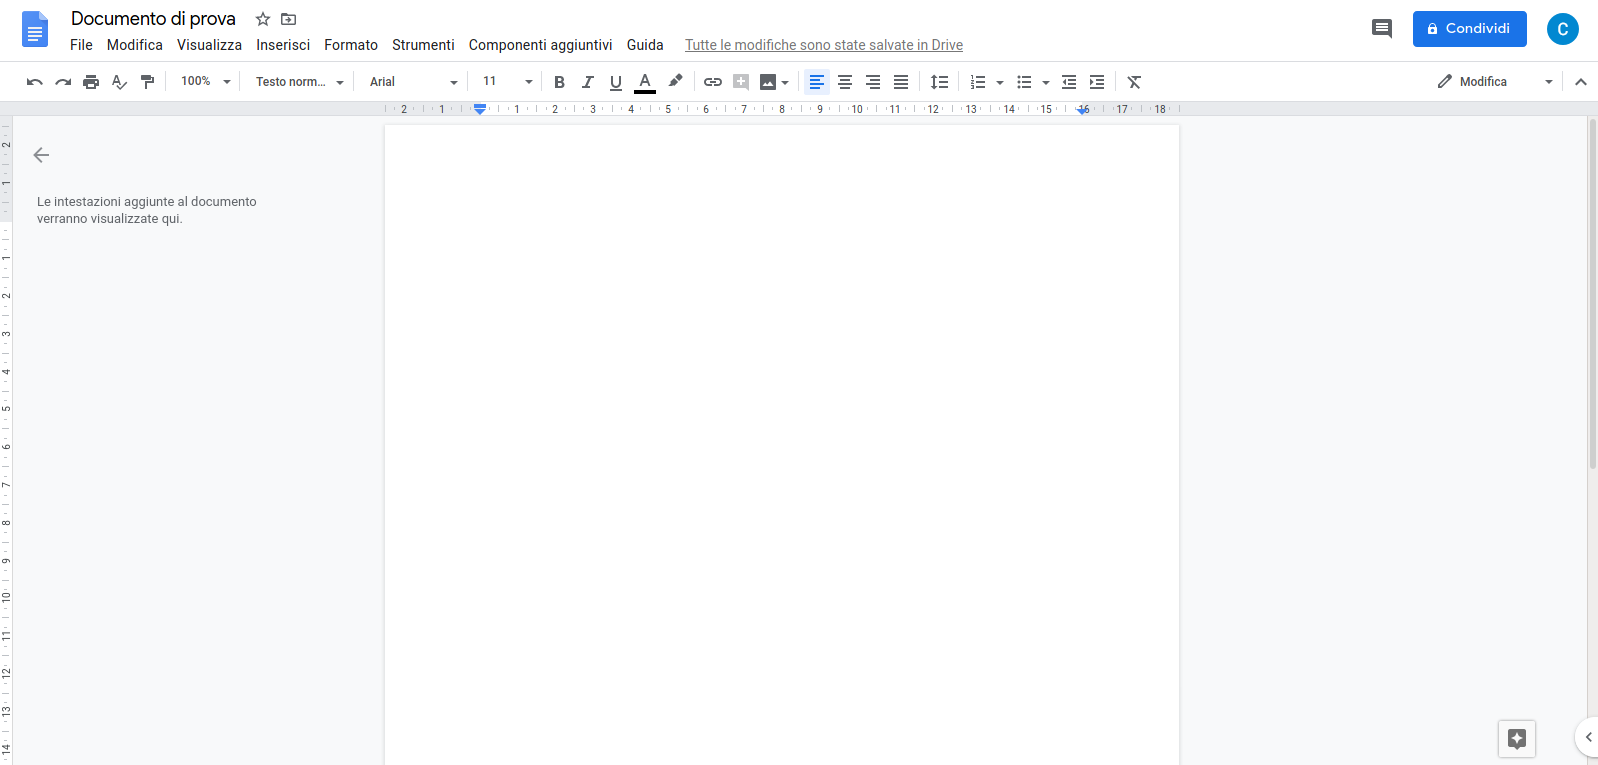
\includegraphics[width=15cm]{img/docs.png}
  \label{fig:github}
  \caption{Google Docs visualizzato nel Browser.}
\end{figure}

\paragraph{Google Drive}
I documenti e le presentazioni sviluppati e redatti durante tutta la durata del progetto sono memorizzati in opportune cartelle pubbliche su Google Drive.


%%%%%%%%%%%%%%%%%%%%%%%%%%%%%%%%%%%%%%%%%%%
%%% 3.2 - GESTIONE DELLA CONFIGURAZIONE %%%
%%%%%%%%%%%%%%%%%%%%%%%%%%%%%%%%%%%%%%%%%%%
\subsection{Gestione della configurazione}
\subsubsection{Scopo}
Lo scopo di questo processo è delineare le norme utili a predisporre il \glossario{workspace} comune per il gruppo; esso definisce anzitutto tutto ciò che concerne il versionamento, comprese la memorizzazione e la manutenzione di quanto prodotto. Descrive inoltre la gestione delle attività che devono essere svolte durante il ciclo di vita del prodotto.

\subsubsection{Aspettative}
L'aspettativa di questo processo coincide con la realizzazione di un ambiente di lavoro usabile e controllato, al fine di semplificare il coordinamento del lavoro tra i diversi componenti del gruppo.

\subsubsection{Attività}
\paragraph{Repository}
Una repository è un ambiente in cui vengono memorizzati, mantenuti e versionati i file di un progetto software, durante il suo intero ciclo di vita. Il sistema di controllo che il gruppo utilizza è \glossario{Git}, e i file dell'intero progetto sono ospitati dalla piattaforma \glossario{Github}; viene inoltre utilizzato \glossario{Git Commitizen} per facilitare il controllo di quanto aggiunto o modificato di volta in volta sulla repository, e \glossario{gitflow} per un più flessibile approccio al lavoro condiviso sulle repository contenenti il codice. \\
I file del progetto sono divisi in tre repository per maggior chiarezza:
\begin{itemize}
  \item \texttt{project-docs}: repository contenente la documentazione;
  \item \texttt{swe-training-app}: repository contenente i sorgenti e i file di configurazione necessari allo sviluppo del programma di addestramento;
  \item \texttt{swe-grafana-plugin}: repository contenente i sorgenti e i file di configurazione necessari allo sviluppo del plug-in di Grafana.
\end{itemize}
Poiché però il prodotto che viene offerto consiste nella somma di software e documentazione, le tre repository sono unite in un'unica repository pubblica contenitrice, chiamata \texttt{swe-predire-in-grafana} e disponibile al seguente indirizzo: \href{https://github.com/CoffeeCodeSWE/swe-predire-in-grafana}{https://github.com/CoffeeCodeSWE/swe-predire-in-grafana}. \\
Tale repository fa uso del meccanismo dei \glossario{git submodules} per combinare più repository in una unica.

\subparagraph{Repository \texttt{project-docs}}
La struttura adottata nella repository \texttt{project-docs} sfrutta il meccanismo di \glossario{branching} offerto dallo strumento Git; questo permette lo sviluppo parallelo di più funzionalità e il lavoro in parallelo sulla stessa repository. \\
La repository utilizzata si suddivide nei seguenti \glossario{branch}:
\begin{itemize}
  \item \texttt{master}: branch principale, sul quale vengono fatte le \glossario{major releases};
  \item \texttt{norme-di-progetto}: branch secondario nel quale viene sviluppato l'intero documento \textsc{Norme di Progetto};
  \item \texttt{analisi-dei-requisiti}: branch secondario nel quale viene sviluppato l'intero documento \textsc{Analisi dei Requisiti};
  \item \texttt{glossario}: branch secondario nel quale viene sviluppato l'intero documento \textsc{Glossario};
  \item \texttt{piano-di-progetto}: branch secondario nel quale viene sviluppato l'intero documento \textsc{Piano di Progetto};
  \item \texttt{piano-di-qualifica}: branch secondario nel quale viene sviluppato l'intero documento \textsc{Piano di Qualifica};
  \item \texttt{studio-di-fattibilita}: branch secondario nel quale viene sviluppato l'intero documento \textsc{Studio di Fattibilità};
  \item \texttt{verbali}: branch secondario nel quale vengono sviluppati i verbali interni ed esterni.
\end{itemize}
Il \glossario{workflow} adottato è basato quindi su un principio della separazione dei documenti: questo, unito ai sistemi anti-collisione di git, permette che, durante il periodo in cui un membro del gruppo è assegnato a un ruolo di redazione specifico, egli sia l'unico a lavorare su tale documento.
\subparagraph*{Struttura dei branch}
Ogni branch è costituito da file, cartelle e sotto-cartelle.
\subparagraph*{File}
I file presenti in ogni branch hanno tipo fisso e predefinito; essi sono:
\begin{itemize}
  \item File di configurazione di Github:
  \begin{itemize}
    \item \texttt{.gitignore}: contiene la lista di file e directory spuri che possono essere presenti nelle repository locali dei componenti del gruppo ma non nella repository remota;
    \item \texttt{README.md}: file markdown contenente una breve descrizione della repository.
  \end{itemize}
  \item File di configurazione di Git Commitizen:
  \begin{itemize}
    \item \texttt{.czcr}: contiene le impostazioni, definite dal gruppo, di Git Commitizen.
  \end{itemize}
  \item File di configurazione di \glossario{Visual Studio Code}
  \begin{itemize}
    \item \texttt{.editorconfig}: contiene le impostazioni, definite dal gruppo, del workspace di Visual Studio Code;
    \item \texttt{settings.json}: contiene le impostazioni specifiche, definite dal gruppo, dell'editor Visual Studio Code;
    \item \texttt{extensions.json}: contiene le estensioni, consigliate per lo sviluppo del progetto, da includere in Visual Studio Code.
  \end{itemize}
  \item File di documentazione:
  \begin{itemize}
    \item File \texttt{.tex}: file \LaTeX\ contenenti il codice sorgente per la generazione dei documenti;
    \item File \texttt{.png} e \texttt{.jpg}: immagini che vengono incluse nei documenti.
  \end{itemize}
\end{itemize}
\subparagraph*{Cartelle}
Ogni branch presenta un insieme di cartelle predefinito:
\begin{itemize}
\item \texttt{.github/}: contiene i file propri di Github;
  \item \texttt{.vscode/}: contiene i file di configurazione di Visual Studio Code;
  \item \texttt{commons/}: contiene i file template di \LaTeX;
  \item \texttt{interni/}: contiene i documenti ad uso interno. In ogni branch questa cartella contiene una sottocartella con lo stesso nome del branch, la quale a sua volta contiene:
  \begin{itemize}
  \item I file sorgente \LaTeX\ dello specifico documento;
  \item Una cartella \texttt{components/}, contenente i subfiles del documento \LaTeX\ principale e una cartella \texttt{img/}, contenente le immagini incluse nel documento.
  \end{itemize}
  \item \texttt{esterni/}: contiene i documenti ad uso esterno. In ogni branch questa cartella contiene una sottocartella con lo stesso nome del branch, la quale a sua volta contiene:
  \begin{itemize}
  \item I file sorgente \LaTeX\ dello specifico documento;
  \item Una cartella \texttt{components/}, contenente i subfiles del documento \LaTeX\ principale e una cartella \texttt{img/}, contenente le immagini incluse nel documento.
  \end{itemize}
\end{itemize}

\subparagraph{Repository \texttt{swe-training-app} e \texttt{swe-grafana-plugin}}
La struttura adottata nelle repositories \texttt{swe-training-app} e \texttt{swe-grafana-plugin} sfrutta il meccanismo di branching in unione al workflow gitflow; questo permette lo sviluppo parallelo di più funzionalità e il lavoro parallelo sulla stessa repository. Le repositories utilizzate si compongono di due branch principali, persistenti durante tutta la durata del progetto:
\begin{itemize}
  \item \texttt{master}: branch principale, aggiornato prima di ogni revisione appena il lavoro necessario all'ingresso in questa è concluso;
  \item \texttt{develop}: branch secondario, aggiornato ad ogni aggiunta di funzionalità o correzione di bug.
\end{itemize}
In aggiunta a questi due branch, un nuovo branch viene creato a partire da \texttt{develop} o \texttt{master} per ogni aggiunta di funzionalità, correzione di bug o rilascio finale del software; per fare ciò viene utilizzato lo strumento gitflow. Ogni nuovo branch segue la seguente nomenclatura:
\begin{center}
  \centering
  \textbf{type/name}
\end{center} dove:
\begin{itemize}
  \item \textbf{type} è il tipo di branch che viene creato. Esso può essere:
  \begin{itemize}
    \item \texttt{feature}: derivato da \texttt{develop} per l'inserimento nella repository di una nuova funzionalità, anche minimale;
    \item \texttt{bugfix}: derivato da \texttt{develop} per la correzione di uno o più bug individuati nel codice;
    \item \texttt{hotfix}: derivato da \texttt{master} per la correzione di uno o più bug individuati nel codice presente nel branch \texttt{master};
    \item \texttt{release}: derivato da \texttt{master}, funge da branch intermedio per la correzione di problemi minori prima del rilascio in produzione.
  \end{itemize}
  \item \textbf{name} è il nome significativo del branch.
\end{itemize}
Al fine di evitare l'introduzione di codice non funzionante o malformato nei branch principali, la due repository fanno ampio uso del meccanismo delle Pull Requests. Ogni qualvolta una funzionalità in un branch secondario viene ultimata, il componente del gruppo responsabile di tale funzionalità ha il compito di aprire una pull request da tale branch verso \texttt{develop}; i verificatori controlleranno quindi la correttezza di quanto aggiunto e provvederanno a eseguire il \glossario{merge} sul branch principale o, nel caso in cui riscontrassero degli errori, a segnalarli tempestivamente all'autore.

\paragraph{Versionamento}
Sebbene il progetto si sviluppi su più repositories, il prodotto che il gruppo deve fornire al proponente deve essere un prodotto unico e coeso; è quindi opportuno che il versionamento dei componenti di questo sia coerente e indichi uno sviluppo complessivo e globale del prodotto. \\
Viene quindi adottato un sistema di versionamento comune a documentazione e componenti software, con delle opportune specializzazioni per entrambi. Un numero di versione di qualsiasi componente si presenta nel seguente modo:
\begin{center}
  \centering
  \textbf{vX.Y-A.B.C-[stato]}
\end{center} dove:
\begin{itemize}
  \item \textbf{vX.Y} indica il procedere globale del prodotto, ed è comune quindi a tutti i componenti nello stesso istante temporale. Nello specifico:
  \begin{itemize}
    \item \textbf{X}: indica il numero di revisione di avanzamento a cui il prodotto si trova. Questa cifra segue le seguenti regole:
    \begin{itemize}
      \item Inizia da 0;
      \item Viene incrementato a ogni superamento di una revisione di avanzamento;
      \item La cifra massima corrisponde al numero massimo di revisioni di avanzamento che il gruppo completerà.
    \end{itemize}
    \item \textbf{Y}: indica il numero di incremento in cui si trova il prodotto. Questa cifra segue le seguenti regole:
    \begin{itemize}
      \item Inizia da 0;
      \item Viene incrementato ad ogni completamento di un incremento, corrispondente a una milestone del progetto;
      \item la cifra massima corrisponde al numero massimo di incrementi previsti dal \textsc{Piano di Progetto}.
    \end{itemize}
  \end{itemize}
  \item \textbf{A.B.C} indica la versione propria del componente singolo. Le cifre da cui è composta questa sezione hanno significato diverso per la documentazione e per il codice, ma in entrambi i casi si segue la logica del \glossario{Semantic Versioning 2.0.0}. Nelle successive sezioni verranno approfondite le regole che queste cifre seguono;
  \item \textbf{[stato]} indica lo stato di sviluppo presso cui si trova un componente software. Anche questa sezione verrà approfondita nelle sezioni successive.
\end{itemize}

\subparagraph{Documenti}
Ogni documento deve essere versionato, al fine di avere una cronologia delle modifiche e una stima dell'importanza di queste sul contenuto del documento. Ad ogni versione del documento corrisponde una riga nel Registro delle modifiche. \\
Il versionamento di un documento segue le regole sopra riportate; il numero di versione di un documento segue quindi il seguente schema:
\begin{center}
  \centering
  \textbf{vX.Y-A.B.C}
\end{center} dove:
\begin{itemize}
  \item \textbf{vX.Y} segue il comportamento sopra riportato;
  \item \textbf{A.B.C}, nel caso specifico dei documenti, assume il seguente significato:
  \begin{itemize}
    \item \textbf{A}: indica un cambiamento radicale nel documento, ossia:
    \begin{itemize}
      \item L'introduzione di un numero di capitoli pari o maggiore a tre;
      \item La rimozione di un numero di capitoli pari o maggiore a tre.
    \end{itemize}
    Questa cifra segue le seguenti regole:
    \begin{itemize}
      \item Inizia da 0;
      \item Viene incrementata ad ogni cambiamento radicale nel documento. L'incremento è ad opera del responsabile o di uno strumento da lui approvato che ne faccia le veci, previa naturalmente la verifica di tutte le sezioni del documento da parte dei verificatori;
      \item Non ha numero massimo e non viene mai resettata.
    \end{itemize}
    \item \textbf{B}: indica un cambiamento importante nel documento, ossia:
    \begin{itemize}
      \item L'introduzione di due o meno capitoli;
      \item La rimozione di due o meno capitoli;
      \item La modifica di uno o più capitoli che abbia ripercussioni sul way of working del gruppo.
    \end{itemize}
    Questa cifra segue le seguenti regole:
    \begin{itemize}
      \item Inizia da 0 ad ogni incremento di A;
      \item Viene incrementata ad ogni cambiamento importante nel documento. L'incremento è ad opera del responsabile o di uno strumento da lui approvato che ne faccia le veci, previa naturalmente la verifica di tutte le sezioni del documento da parte dei verificatori;
      \item Non ha numero massimo.
    \end{itemize}
    \item \textbf{C}: indica un cambiamento generico nel documento, ossia:
    \begin{itemize}
      \item La modifica di una piccola parte di documento;
      \item Lo spostamento di una sezione in un'altra posizione dello stesso documento;
      \item Una correzione di tipo ortografico o grammaticale.
    \end{itemize}
    Questa cifra segue le seguenti regole:
    \begin{itemize}
      \item Inizia da 0 ad ogni incremento di B o A;
      \item Viene incrementata ad ogni cambiamento generico nel documento. L'incremento è ad opera di un verificatore.
      \item Non ha numero massimo.
    \end{itemize}
  \end{itemize}
\end{itemize}


\subparagraph{Componenti software}
Al pari della documentazione, anche i file delle componenti software del prodotto devono essere versionati. \\
Il versionamento del codice segue le regole sopra riportate; il numero di versione di un componente software segue quindi il seguente schema:
\begin{center}
  \centering
  \textbf{vX.Y-A.B.C-stato}
\end{center} dove:
\begin{itemize}
  \item \textbf{vX.Y} segue il comportamento sopra riportato;
  \item \textbf{A.B.C}, nel caso specifico dei componenti software, assume il seguente significato:
  \begin{itemize}
    \item \textbf{A}: corrisponde a una \glossario{Major Release}, e indica quindi l'implementazione di tutti i requisiti richiesti. Questa cifra segue le seguenti regole:
    \begin{itemize}
      \item Inizia da 0;
      \item Viene incrementata al completamento di tutti i requisiti richiesti.
    \end{itemize}
    \item \textbf{B}: corrisponde a una \glossario{Minor Release}, e indica quindi l'implementazione di uno o più requisiti richiesti. Questa cifra segue le seguenti regole:
    \begin{itemize}
      \item Inizia da 0 a ogni incremento di A;
      \item Viene incrementata al completamento di uno o più requisiti;
      \item La cifra massima corrisponde al massimo numero di requisiti riportati nell'\textsc{Analisi dei Requisiti}.
    \end{itemize}
    \item \textbf{C}: corrisponde a una \glossario{Patch}, e indica quindi la modifica a uno o più requisiti. Questa cifra segue le seguenti regole:
    \begin{itemize}
      \item Iniza da 0 ad ogni incremento di B o di A;
      \item Viene incrementata alla modifica verificata di uno o più requisiti;
      \item Non ha numero massimo.
    \end{itemize}
  \end{itemize}
  \item \textbf{stato} indica lo stato a cui si trova il software, il quale può essere:
  \begin{itemize}
    \item \textbf{stable}: software stabile e che soddisfa tutti i requisiti, pronto ad essere rilasciato in produzione;
    \item \textbf{rc}: \textit{release candidate}, ossia software funzionante e che soddisfa gran parte dei requisiti, pronto per essere rilasciato dopo qualche lieve miglioria;
    \item \textbf{dev}: ancora in via di sviluppo. Software funzionante ma ancora incompleto.
  \end{itemize}
\end{itemize}

\paragraph{Continuous Integration}
Il gruppo fa uso della pratica di \glossario{Continuous Integration} al fine di ottenere un prodotto sempre funzionante, anche se composto da singole componenti sviluppate da persone diverse. Nello specifico, le repository contententi codice sorgente implementeranno questa pratica con l'utilizzo di due strumenti:
\begin{itemize}
  \item \textbf{\glossario{Sonarcloud}} per l'analisi statica del codice (\glossario{Continuous Inspection});
  \item \textbf{\glossario{Travis CI}} per le operazioni di controllo basate sui test definiti nel \textsc{Piano di Qualifica v2.0.0} e il supporto al versionamento dei documenti e delle componenti software.
\end{itemize}

\subsubsection{Strumenti}
Le attività di gestione della configurazione sono coadiuvate dall'utilizzo di strumenti software, che permettono il perseguimento del giusto workflow e l'applicazione delle norme.
\paragraph{Git}
La repository è ospitata dal servizio di \glossario{hosting} Github; per operare sulla repository vengono utilizzati tre strumenti:
\begin{itemize}
  \item Portale Github.com;
  \item Git Commitizen;
  \item Visual Studio Code.
\end{itemize}
\paragraph{Portale Github.com}
Il portale Github.com permette la consultazione immediata di quanto fatto e pubblicato, e la gestione delle \glossario{issues} e delle \glossario{milestones}.
\begin{figure}[H]
  \centering
  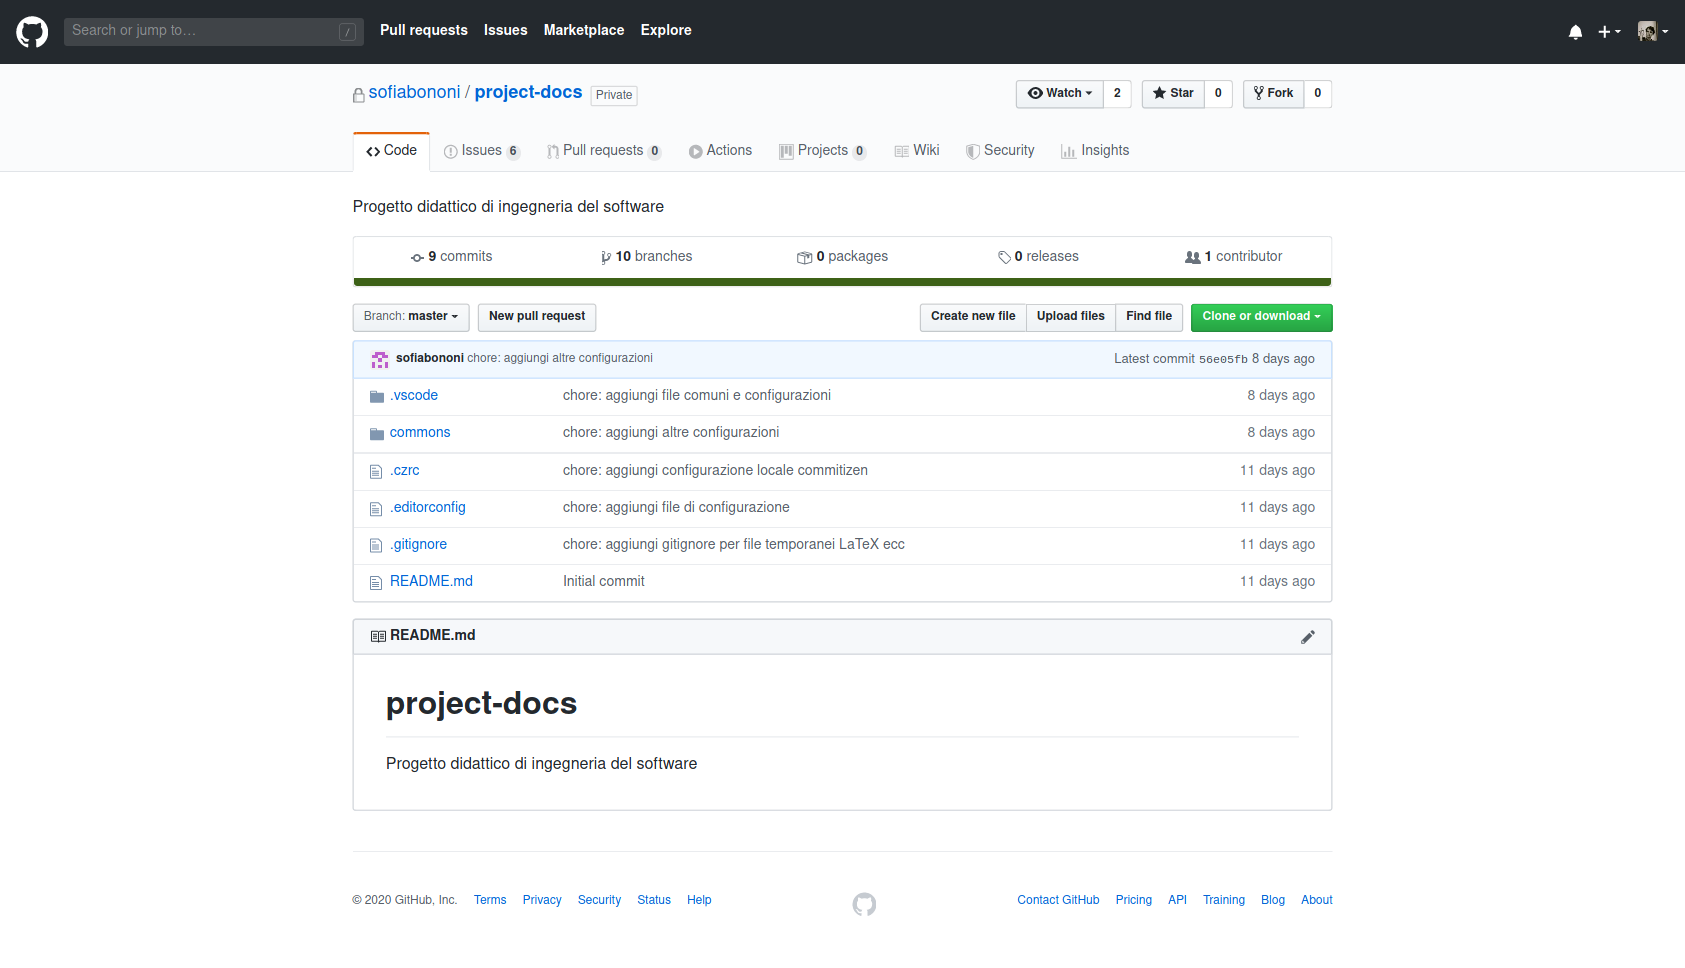
\includegraphics[width=15cm]{img/github.png}
  \label{fig:github}
  \caption{Portale in Github della repository di progetto.}
\end{figure}

\paragraph{Git Commitizen}
Per il \glossario{commit} delle modifiche ai file della repository viene utilizzato Git Commitizen tramite Command Line, il quale assicura l'uniformità dei commit e quindi una maggiore chiarezza di quanto viene versionato. \\ Questo strumento permette di compilare in maniera guidata e uniforme il messaggio di commit, richiedendo nell'ordine:
\begin{itemize}
  \item Il tipo di commit che viene eseguito; questo può essere:
  \begin{itemize}
    \item \textbf{feat}: l'aggiunta di una nuova feature;
    \item \textbf{fix}: il fix di un bug;
    \item \textbf{docs}: un cambiamento riguardante esclusivamente la documentazione;
    \item \textbf{style}: un cambiamento che non modifica il significato del codice, ad esempio piccoli cambi di formattazione;
    \item \textbf{refactor}: un cambiamento nel codice che non risolve un bug e che non aggiunge una nuova feature;
    \item \textbf{perf}: un cambiamento nel codice che migliora le performance;
    \item \textbf{test}: l'aggiunta di test mancanti;
    \item \textbf{chore}: uno o più cambiamenti al processo di build, a strumenti ausiliari o a \glossario{librerie}.
  \end{itemize}
  \item Quali sono i files della repository coinvolti nel cambiamento (opzionale);
  \item Una descrizione breve del cambiamento, scritta in prima persona imperativo;
  \item Una descrizione più lunga del cambiamento (opzionale);
  \item Se il cambiamento fatto è importante o marginale (scelta sì/no);
  \item Se il cambiamento coinvolge una o più issues aperte.
\end{itemize}
\paragraph{Git submodules}
Il meccanismo dei Git submodules consiste nel collegamento di più repository in un'unica repository contenitrice. In questa, le diverse repository del progetto vengono collegate tramite un puntatore all'ultimo commit eseguito su ogni repository, risultando così come singole cartelle.

\paragraph{Gitflow}
Il gruppo utilizza lo strumento gitflow per la creazione di branch \textit{ad hoc}, seguendo le regole precedentemente descritte.

\paragraph{Sonarcloud}
La repository \texttt{swe-code} integra lo strumento di Continuous Inspection Sonarcloud; questo permette l'analisi automatica del codice creato ogniqualvolta viene aperta una Pull Request da un branch secondario a un branch principale. \\
Lo strumento identifica:
\begin{itemize}
  \item Eventuali bug nel codice;
  \item Eventuali vulnerabilità di sicurezza;
  \item Eventuali ripetizioni di codice;
  \item Eventuali \textit{code smells}, ossia indicatori di una cattiva scrittura del codice che possono in futuro portare ad errori o cali di performance.
\end{itemize}

\paragraph{Travis CI}
Travis CI è un servizio di Continuous Integration (CI) utilizzato per il \glossario{build} e il testing di prodotti software. Questo strumento viene utilizzato dal gruppo per il processo di Continuous Integration implementato nelle repository contententi codice sorgente.

\paragraph{Visual Studio Code}
Due estensioni di Visual Studio Code permettono di operare sulla repository:
\begin{itemize}
  \item \textbf{Git Graph}: visualizzazione del grafo della repository e possibilità di svolgere azioni Git direttamente su di esso;
  \item \textbf{GitHub Pull Requests}: strumento di revisione delle \glossario{Pull Requests} di Github.
\end{itemize}

\begin{figure}[H]
  \centering
  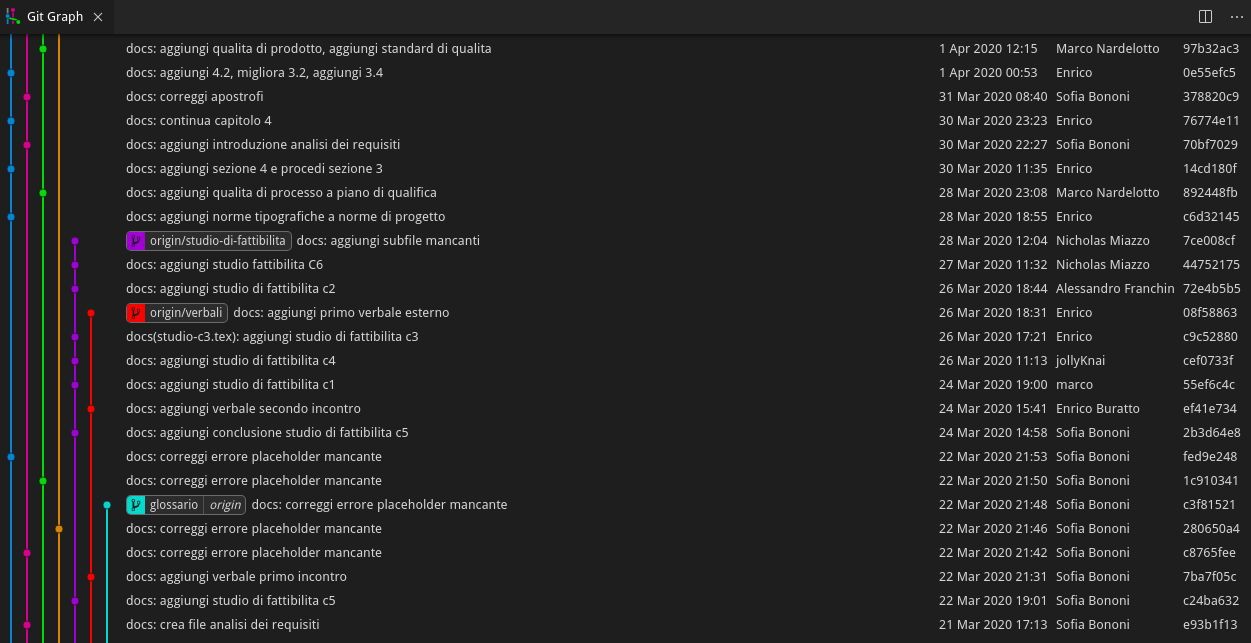
\includegraphics[width=15cm]{img/gitgraph.png}
  \label{fig:github}
  \caption{Estensione Git Graph nell'IDE Visual Studio Code.}
\end{figure}

%%%%%%%%%%%%%%%%%%%%%%%%%%%%%%%%%%%%%%
%%% 3.3 - GESTIONE DEI CAMBIAMENTI %%%
%%%%%%%%%%%%%%%%%%%%%%%%%%%%%%%%%%%%%%
\subsection{Gestione dei cambiamenti}
\subsubsection{Scopo}
Lo scopo del processo di gestione dei cambiamenti è fornire un mezzo tempestivo e documentato che assicuri che tutti i problemi vengano individuati, documentati e risolti.

\subsubsection{Aspettative}
Le aspettative di questo processo sono:
\begin{itemize}
  \item L'individuazione di un metodo efficace per trovare e correggere gli errori;
  \item L'ottenimento di un tracciamento continuo degli errori più comuni e delle loro cause.
\end{itemize}
L'obiettivo finale è quindi la persecuzione di una qualità più elevata nella documentazione e nel codice.

\subsubsection{Descrizione}
Questo processo fornisce una linea guida univoca per l'analisi, il tracciamento e la rimozione dei problemi sorti durante lo svolgimento del progetto.

\subsubsection{Attività}
\paragraph{Implementazione del processo}
Il processo di gestione dei cambiamenti viene eseguito ogni volta si renda necessario per la comparsa di un problema; esso dovrà rispettare i seguenti requisiti:
\begin{itemize}
  \item Dovrà essere un ciclo chiuso, assicurandosi che:
  \begin{itemize}
    \item Tutti i problemi individuati vengano prontamente segnalati e immessi nel processo di gestione dei cambiamenti;
    \item L'azione correttiva venga inizializzata;
    \item Le parti interessate siano appropriatamente avvisate dell'esistenza del problema;
    \item Le cause vengano identificate, analizzate e, possibilmente, rimosse.
  \end{itemize}
  \item Il processo deve rispettare uno schema per categorizzare e dare priorità ai problemi;
  \item Devono essere effettuate delle analisi per rilevare la presenza di tendenze nei problemi riportati;
  \item Il processo di risoluzione dei problemi deve essere valutato; si valuterà:
  \begin{itemize}
    \item La risoluzione effettiva dei problemi;
    \item L'annullamento delle eventuali tendenze;
    \item La non-introduzione di nuovi errori.
  \end{itemize}
\end{itemize}
Il processo farà uso di uno schema di categorizzazione dei cambiamenti, consistente di quattro voci:
\begin{itemize}
  \item \textbf{ID}: numero identificativo univoco del cambiamento;
  \item \textbf{Processo}: il processo nel quale è stato individuato il problema;
  \item \textbf{Osservazione}: osservazione del problema, svolta dal proponente, dal committente o da un membro del gruppo;
  \item \textbf{Soluzione}: la soluzione intrapresa per risolvere o mitigare il problema.
\end{itemize}
Il numero identificativo è codificato nel seguente modo: \\
\begin{center}
  \centering
  \textbf{CM[P][N]}
\end{center} dove:
\begin{itemize}
  \item \textbf{P} è la priorità del problema, la quale può essere:
  \begin{itemize}
    \item \textbf{A}: alta, richiede una risoluzione immediata;
    \item \textbf{M}: media, ossia non urgente ma con un'alta probabilità di degenerare nel tempo;
    \item \textbf{B}: bassa, ossia non urgente e con una bassa probabilità di degenerare nel tempo.
  \end{itemize}
  \item \textbf{N} è il numero progressivo, il quale segue le seguenti regole:
  \begin{itemize}
    \item Parte da 1;
    \item Viene incrementato a ogni introduzione di un cambiamento;
    \item Non ha limite massimo.
  \end{itemize}
\end{itemize}

\paragraph{Risoluzione dei problemi}
Lo schema individuato segue lo schema fornito dalle GitHub Issues; ogniqualvolta un problema venga individuato, esso deve essere segnalato tramite \textit{issue}, la quale deve comprendere:
\begin{itemize}
  \item Un titolo e una descrizione del problema, comprendenti il codice identificativo;
  \item Uno o più assegnatari incaricati della risoluzione del problema;
  \item Un'etichetta che identifichi la tipologia del problema.
\end{itemize}
Una volta risolto il problema, l'assegnatario finale provvederà a chiudere la issue tramite commento di commit, in modo da tenerne tracciata anche la chiusura.

\subsubsection{Strumenti}
\paragraph{GitHub Issues}
Il gruppo fa uso delle GitHub Issues per il tracciamento dei problemi. Questo strumento è integrato in GitHub, già usato dal gruppo come sede delle repository del progetto; tra le molte funzionalità messe a disposizione, spiccano per utilità la possibilità di associare ogni \textit{issue} a un determinato commit e di assegnare uno o più componenti ad ogni \textit{issue}.

%%%%%%%%%%%%%%%%%%%%%%%%%%%%%%%%%%%%a
%%% 3.4 - GESTIONE DELLA QUALITÀ %%%
%%%%%%%%%%%%%%%%%%%%%%%%%%%%%%%%%%%%
\subsection{Gestione della qualità}
\subsubsection{Scopo}
Lo scopo del processo di gestione della qualità è garantire che i prodotti software e i processi del ciclo di vita siano conformi ai requisiti concordati con il cliente, e che rispettino gli obiettivi di qualità.
\subsubsection{Aspettative}
Le aspettative di questo processo sono le seguenti:
\begin{itemize}
  \item Ottenere qualità nell'organizzazione;
  \item Sviluppare un prodotto software di qualità, comprendente anche una documentazione completa e di facile fruizione.
\end{itemize}
\subsubsection{Descrizione}
La gestione della qualità viene trattata nello specifico nel \textsc{Piano di Qualifica}. In particolare, in tale documento:
\begin{itemize}
  \item Sono presentati gli standard di qualità utilizzati;
  \item Di tali standard, sono individuati i processi di interesse per il particolare progetto.
\end{itemize}
Per ogni processo vengono descritti:
\begin{itemize}
  \item Le funzioni di tale processo;
  \item Le metriche da utilizzare;
  \item Gli obiettivi che tale processo persegue.
\end{itemize}
Per ogni prodotto, invece, vengono descritti:
\begin{itemize}
  \item Le metriche da utilizzare;
  \item Gli obiettivi da perseguire.
\end{itemize}
\subsubsection{Attività}
\paragraph{Classificazione dei processi}
I processi sono codificati in tal modo: \\
\begin{center}
  \centering
  \textbf{PRC[ID][Nome]}
\end{center} dove:
\begin{itemize}
  \item \textbf{PRC} indica "Processo";
  \item \textbf{ID} è un indicatore numerico a tre cifre;
  \item \textbf{Nome} è il riassunto della funzione del processo.
\end{itemize}

Gli obiettivi di qualità dei processi vengono codificati in tal modo: \\
\begin{center}
  \centering
  \textbf{QoPR[ID][Nome]}
\end{center} dove:
\begin{itemize}
  \item \textbf{QoPR} indica \textit{Quality of process};
  \item \textbf{ID} è un indicatore numerico a tre cifre;
  \item \textbf{Nome} è il riassunto della descrizione del processo.
\end{itemize}

\subparagraph{Metriche di qualità dei processi}
Le metriche di qualità dei processi sono codificate in tal modo: \\
\begin{center}
  \centering
  \textbf{MoPR[ID][Nome]}
\end{center} dove:
\begin{itemize}
  \item \textbf{QoPR} indica \textit{Metric of process};
  \item \textbf{ID} è un indicatore numerico a tre cifre;
  \item \textbf{Nome} è il riassunto della descrizione della metrica.
\end{itemize}

\paragraph{Classificazione di qualità dei prodotti}
Gli obiettivi di qualità dei prodotti sono codificati nel seguente modo: \\
\begin{center}
  \centering
  \textbf{QoPD[ID][Nome]-[Caratteristica]}
\end{center} dove:
\begin{itemize}
  \item \textbf{QoPD} indica \textit{Quality of product};
  \item \textbf{ID} è un indicatore numerico a tre cifre;
  \item \textbf{Nome} è il riassunto della descrizione del processo;
  \item \textbf{Caratteristica} indica a quale caratteristica appartiene l'obiettivo.
\end{itemize}

\subparagraph{Metriche di qualità dei prodotti}
Le metriche di qualità dei prodotti sono codificate nel seguente modo:
\begin{center}
  \centering
  \textbf{MoPD[ID][Nome]-[Caratteristica]}
\end{center} dove:
\begin{itemize}
  \item \textbf{MoPD} indica \textit{Metric of product};
  \item \textbf{ID} è un indicatore numerico a tre cifre;
  \item \textbf{Nome} è il riassunto della descrizione della metrica;
  \item \textbf{Caratteristica} indica a quale caratteristica appartiene la metrica.
\end{itemize}

%%%%%%%%%%%%%%%%%%%%%%
%%% 3.5 - VERIFICA %%%
%%%%%%%%%%%%%%%%%%%%%%
\subsection{Verifica}

\subsubsection{Scopo}
Lo scopo del processo di verifica è quello di verificare che il prodotto venga realizzato nel modo corretto, secondo delle regole stabilite. \\
Il processo di verifica interessa sia il software che la documentazione prodotta, assicurando che il prodotto finale sia corretto e completo.

\subsubsection{Aspettative}
La procedura che tale processo, al fine di essere implementato correttamente, deve rispettare, è la seguente:
\begin{itemize}
  \item Vengono definiti dei chiari criteri di accettazione;
  \item Vengono definite delle attività di verifica, con relativa documentazione;
  \item Vengono eseguiti dei test di verifica, ed eventuali difetti vengono catalogati;
  \item Eventuali difetti vengono corretti.
\end{itemize}

\subsubsection{Descrizione}
Il processo di verifica inizia con un prodotto del quale è necessario controllare la conformità alle aspettative e finisce con un prodotto che le soddisfa. Una volta verificato, il prodotto passerà alla fase di validazione.

\subsubsection{Attività}
Le attività di questo processo sono di due tipologie:
\begin{itemize}
  \item Analisi;
  \item Test.
\end{itemize}
\paragraph{Analisi}
L'attività di analisi si divide in due sottocategorie:
\begin{itemize}
  \item Analisi Statica;
  \item Analisi Dinamica.
\end{itemize}
\subparagraph{Analisi Statica}
L'analisi statica è l'attività di analisi che viene eseguita sul prodotto senza il bisogno che questo venga eseguito. Essa valuta la presenza o assenza di errori e/o difetti, la conformità alle regole definite e la coesione dei componenti. \\
L'analisi statica si divide in due tipologie:
\begin{itemize}
  \item \textbf{\glossario{Walkthrough}}: i componenti del gruppo analizzano il prodotto nella sua interezza alla ricerca di difetti e di inconformità con le regole prescritte. Questa tecnica verrà utilizzata più intensamente durante l'inizio del progetto, per lasciare il tempo ai vari componenti di familizzare con le norme prescritte. Durante questa attività viene stipulata una lista di controllo contenente gli errori trovati;
  \item \textbf{\glossario{Inspection}}: questa tipologia di analisi statica viene eseguita dal singolo verificatore, che provvederà a ricercare gli errori segnalati nella lista di controllo all'interno di quanto prodotto; è quindi un'analisi più precisa e mirata agli errori che vengono più comunemente commessi.
\end{itemize}
Segue la lista di controllo parziale, contenente gli errori più comuni finora trovati. Questa lista verrà possibilmente ampliata al progredire degli eventuali errori trovati.

\begin{table}[H]
\centering
\begin{tabular}{p{5cm}p{10cm}}
\textbf{Oggetto}           & \textbf{Controllo da effettuare}      \\
Data e ora                              & Verificare il giusto formato: deve essere coerente con lo standard ISO 8601 \\
Sintassi                          & Verificare che le frasi non siano eccessivamente verbose o sintatticamente errate       \\
Uniformità nell'utilizzo dei termini & Controllare che i termini ambigui vengano usati uniformemente (\underline{e.g.} \textit{obiettivo}-\textit{obbiettivo}) \\
Nidificazione sezioni            & Verificare che non vi siano incongruenze nella nidificazione delle varie sezioni, cioè: \begin{itemize}
  \item Le sezioni, capitoli, paragrafi e sottoparagrafi abbiano numerazione non crescente;
  \item Non venga utilizzato il giusto ordine di indentazione.
\end{itemize}       \\
Elenchi                           & \begin{itemize}
  \item Verificare che la prima lettera di ogni elemento sia maiuscola;
  \item Verificare che ogni elemento finisca con la corretta punteggiatura (; o .).
\end{itemize}       \\
\end{tabular}
\caption{Errori frequenti nella documentazione.}
\end{table}

\subparagraph{Analisi Dinamica}
L'analisi dinamica è la tipologia di analisi che viene eseguita sul prodotto eseguendolo. Essa viene effettuata tramite dei test, che controllano il corretto funzionamento del prodotto.

\paragraph{Test}
L'attività di test fa parte dell'analisi dinamica; i test hanno come scopo principale la verifica del corretto funzionamento del codice, individuando eventuali errori di funzionamento. \\
Per la corretta implementazione dei test, essi devono essere automatizzati e ripetibili; devono essere definiti a tale scopo:
\begin{itemize}
  \item L'ambiente di sviluppo, ossia il sistema sul quale viene eseguito il test;
  \item Lo stato iniziale;
  \item I dati di input;
  \item I dati di output attesi;
  \item Le istruzioni che vengono eseguite.
\end{itemize}
I test appartengono a diverse categorie; essi possono essere infatti:
\begin{itemize}
  \item Test di unità;
  \item Test di regressione;
  \item Test di integrazione;
  \item Test di sistema.
\end{itemize}

\subparagraph*{Test di unità}
I test di unità sono quelli più piccoli in granularità: un test di unità testa infatti il funzionamento di una componente individuale del prodotto. Essendo queste ultime in gran numero, è opportuno sfruttare al massimo il parallelismo, in modo da eseguirne un gran numero contemporaneamente; per lo stesso motivo, il test delle unità più semplici è a cura dello stesso programmatore.

\subparagraph*{Test di regressione}
Il test di regressione comprende tutti i test che accertano che la modifica di un componente del sistema non vada a influenzare, causando errori, alcuna altra parte in relazione con essa. Essi vengono quindi eseguiti ogni volta che un'unità viene modificata, per assicurare che il cambiamento non induca una regressione di quanto fatto. \\
A questo scopo, vengono quindi rieseguiti tutti i test delle componenti interessate.

\subparagraph*{Test di integrazione}
I test di integrazione testano il sistema dopo l'assemblamento di più componenti sviluppati in parallelo; essi assicurano quindi il corretto funzionamento di tutte queste componenti nel loro insieme. \\
I test di integrazione vengono codificati nel seguente modo:
\begin{center}
  \centering
  \textbf{TI-[N]}
\end{center} dove:
\begin{itemize}
  \item \textbf{TI} indica Test di Sistema;
  \item \textbf{N} indica un numero progressivo che parte da 1.
\end{itemize}

\subparagraph*{Test di sistema}
Attraverso i test di sistema, l'intero sistema viene testato nella sua interezza, una volta cioè integrati tutti i componenti. \\
I Test di sistema vengono codificati nel seguente modo:
\begin{center}
  \centering
  \textbf{TS[Id]}
\end{center} dove:
\begin{itemize}
  \item \textbf{TS} indica Test di Sistema;
  \item \textbf{Id} si riferisce alla codifica del requisito funzionale al quale il test di sistema si applica.
\end{itemize}

%METRICHEPDQ4
\subsubsection{Metriche}
\paragraph{PRC004 Verifica}
Questo processo farà uso delle seguenti metriche:
\begin{itemize}
  \item MoPR012 Frequenza dei controlli;
  \item MoPR013 Percentuale di test soddisfatti.
\end{itemize}
\subparagraph{MoPR012 Frequenza dei controlli}
\begin{itemize}
  \item \textbf{Descrizione}: i verificatori devono costantemente controllare l'andamento dello sviluppo dei prodotti e validarli secondo le norme.
\end{itemize}

\subparagraph{MoPR013 Percentuale di test soddisfatti}
\begin{itemize}
  \item \textbf{Descrizione}: questa metrica identifica la percentuale di test implementati e soddisfatti tra quelli definiti dal gruppo nel \textsc{Piano di Qualifica}.
  \item \textbf{Unità di misura}: percentuale;
  \item \textbf{Formula}: la formula per tale metrica è la seguente:
  \begin{displaymath}
    \frac{\#TI * 100}{\#TT}
  \end{displaymath}
  dove:
  \begin{itemize}
    \item $ \#TI $: numero di test implementati;
    \item $ \#TT $: numero totale di test documentati.
  \end{itemize}
\end{itemize}

%%%%%%%%%%%%%%%%%%%%%%%%%
%%% 3.6 - VALIDAZIONE %%%
%%%%%%%%%%%%%%%%%%%%%%%%%
\subsection{Validazione}
\subsubsection{Scopo}
Lo scopo del processo di validazione è determinare se il prodotto soddisfa i requisiti concordati con il proponente e l'utilizzo specifico per cui è stato creato. Questo processo esegue quindi il test completo sul sistema, assicurando infine che le necessità del cliente siano state pienamente soddisfatte. \\ Il processo di validazione viene effettuato dopo il processo di verifica, per avere la certezza che tutte le componenti del sistema possano essere verificate.
\subsubsection{Attività}
Il processo di validazione consiste delle seguenti attività:
\begin{itemize}
  \item Individuare una strategia di validazione, comprendente:
  \begin{itemize}
    \item L'identificazione degli oggetti da validare;
    \item L'identificazione delle attività di valutazione da applicare.
  \end{itemize}
  \item Eseguire la strategia, ovverosia svolgere la validazione;
  \item Valutare i risultati ottenuti dalla strategia:
  \begin{itemize}
    \item Se i risultati sono positivi vengono consegnati al proponente;
    \item Se lo svoglimento dell'attività presenta problemi o inconformità con le richieste del cliente, questi devono essere risolti e, successivamente, i risultati devono essere consegnati al proponente.
  \end{itemize}
\end{itemize}
\paragraph{Test}
Nel processo di validazione vengono eseguiti i test di accettazione, i quali corrispondono con i test di sistema con la differenza che essi vengono eseguiti con il supervisionamento del committente per dimostrare la conformità del prodotto con quanto richiesto; essi quindi accertano la copertura dei requisiti software concordati con il proponente.
\end{document}
